\section{Model Design and Fitting}

\subsection{Model choose and hyperparameter tuning}

In this study, we employed two well-known supervised learning algorithms—K-nearest neighbors (KNN) and 
Random Forest—to predict patients' levels of disability. These models were chosen for their contrasting characteristics:
KNN is a simple, non-parametric classifier that predicts based on the majority label of its nearest neighbors, 
while Random Forest is an ensemble learning method renowned for its robustness, decorrelation between trees, 
and ability to handle high-dimensional datasets. 

Both KNN and Random Forest rely on hyperparameters that can significantly influence predictive performance.
To optimize these parameters, we utilized k-fold cross-validation as the primary evaluation method. 
This approach divides the training data into k folds, iteratively training the model on k–1 
folds and validating it on the remaining fold. This process reduces overfitting and provides
a more reliable estimate of model performance. For the Random Forest algorithm,
we further employed grid search to systematically explore multiple hyperparameter combinations.
Throughout the tuning process, accuracy was used as the evaluation metric for selecting the best-performing hyperparameters,
given its simplicity and effectiveness in classification tasks. This ensured fair and consistent comparisons across models and datasets.

The hyperparameter tuning process was conducted independently for each model on four datasets: the raw,
randomly oversampled, SMOTE-balanced, and advanced-balanced datasets. 
For the KNN algorithm, the most critical hyperparameter is k, which defines the number of nearest
neighbors considered during prediction. To identify the optimal k value, we evaluated a range from
1 to 30 using cross-validation and selected the value that yielded the highest accuracy.
As shown in the plots below, k = 25 was optimal for the original (imbalanced) dataset, while k = 1 performed
best for the random oversampling, SMOTE-balanced, and advanced-balanced datasets.
This suggests that balancing the data reduces the need to aggregate across neighbors,
    enabling the model to better capture localized patterns.


\begin{figure}[!h]
    \centering
    \begin{subfigure}[t]{0.45\textwidth}
        \centering
        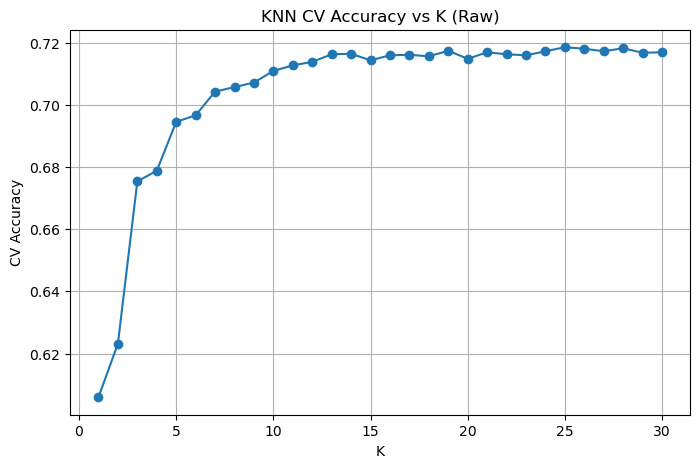
\includegraphics[width=\textwidth]{../results/knn_cs_k_raw.png}
        \caption{KNN hyperparameter tuning for the original dataset.}
        \label{fig:knn_k_tuning_raw}
    \end{subfigure}
    \hfill
    \begin{subfigure}[t]{0.45\textwidth}
        \centering
        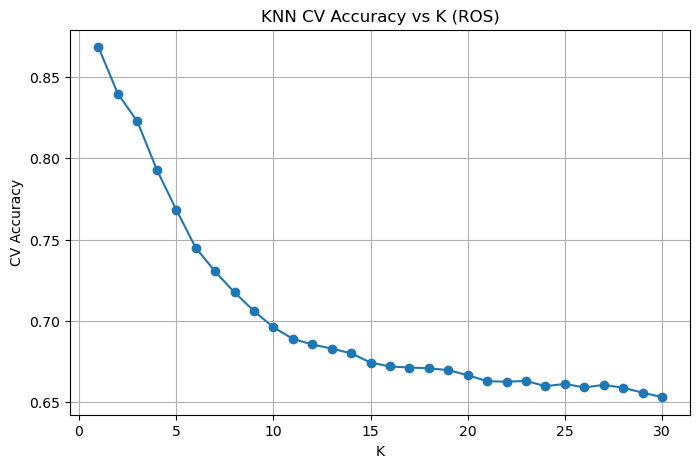
\includegraphics[width=\textwidth]{../results/knn_vs_k_ros.png}
        \caption{KNN hyperparameter tuning for the random oversampling dataset.}
        \label{fig:knn_k_tuning_ros}
    \end{subfigure}
    \vskip\baselineskip
    \begin{subfigure}[t]{0.45\textwidth}
        \centering
        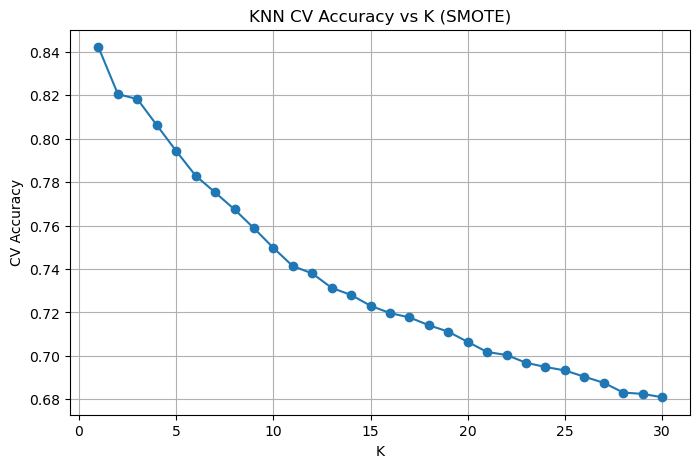
\includegraphics[width=\textwidth]{../results/knn_vs_k_smote.png}
        \caption{KNN hyperparameter tuning for the SMOTE-balanced dataset.}
        \label{fig:knn_k_tuning_smote}
    \end{subfigure}
    \hfill
    \begin{subfigure}[t]{0.45\textwidth}
        \centering
        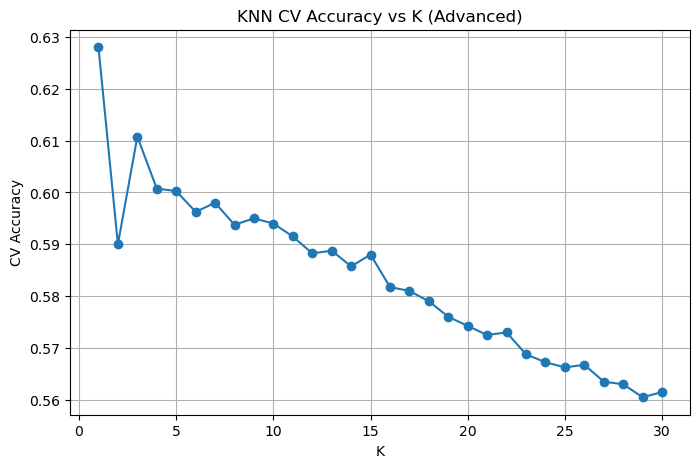
\includegraphics[width=\textwidth]{../results/knn_vs_k_advanced.png}
        \caption{KNN hyperparameter tuning for the advanced-balanced dataset.}
        \label{fig:knn_k_tuning_advanced}
    \end{subfigure}
    \caption{KNN hyperparameter tuning results for different datasets.}
    \label{fig:knn_hyperparameter_tuning}
\end{figure}


\section{Random Forest Optimization and Comparative Evaluation}

\subsection{Hyperparameter Tuning}

\subsection{Random Forest Hyperparameter Tuning}

In Random Forest, different hyperparameters need to be set and evaluated to achieve optimal model performance. Key hyperparameters include the number of trees in the forest (\texttt{n\_estimators}), the number of features considered at each split (\texttt{max\_features}), the maximum depth of each tree (\texttt{max\_depth}), the maximum number of leaf nodes (\texttt{max\_leaf\_nodes}), and the minimum number of samples required at each node (\texttt{min\_samples\_leaf}).

Due to the large number of possible hyperparameter combinations, we applied grid search combined with cross-validation to identify the best-performing configurations. 
A range of values was specified for each parameter. Specifically:

\begin{itemize}
    \item \texttt{n\_estimators}: \{50, 100, 200, 300, 500, 1000\}
    \item \texttt{max\_features}: from 1 to the total number of predictors
    \item \texttt{max\_depth}: \{5, 10, 15, 20, 30, Unlimited\}
    \item \texttt{max\_leaf\_nodes}: \{10, 20, 50, Unlimited\}
    \item \texttt{min\_samples\_leaf}: \{1, 2, 5, 10\}
\end{itemize}

Based on the cross-validation results, the optimal hyperparameter combinations that achieved the 
highest validation accuracy are summarized in Table~\ref{tab:rf_hyperparameters}.
 These findings suggest that different data balancing methods can influence the ideal model complexity and tree structure required for best predictive performance.

    
\begin{table}[!h]
    \centering
    \resizebox{\textwidth}{!}{%
    \begin{tabular}{|l|c|c|c|c|c|}
    \hline
    \textbf{Dataset} & \texttt{n\_estimators} & \texttt{max\_features} & \texttt{max\_depth} & \texttt{max\_leaf\_nodes} & \texttt{min\_samples\_split} \\
    \hline
    Raw & 100 & 6 & 10 & 50 & 1 \\
    Random Oversampling & 300 & 4 & 30 & Unlimited & 1 \\
    SMOTE & 300 & 4 & 30 & Unlimited & 1 \\
    Advanced Sampling & 300 & 4 & 30 & Unlimited & 1 \\
    \hline
    \end{tabular}%
    }
    \caption{Optimal hyperparameters for Random Forest across different datasets.}
    \label{tab:rf_hyperparameters}
\end{table}

\section{Results}

Models were trained and evaluated using accuracy, sensitivity (recall), and specificity:

\begin{align*}
\text{Accuracy} &= \frac{TP + TN}{TP + TN + FP + FN} \\
\text{Sensitivity (Recall)} &= \frac{TP}{TP + FN} \\
\text{Specificity} &= \frac{TN}{TN + FP}
\end{align*}

\subsection{Raw Dataset}

\begin{table}[!h]
\centering
\resizebox{\textwidth}{!}{%
\begin{tabular}{|l|ccc|ccc|ccc|ccc|ccc|}
\hline
\textbf{Model} & \multicolumn{3}{c|}{Class 1} & \multicolumn{3}{c|}{Class 2} & \multicolumn{3}{c|}{Class 3} & \multicolumn{3}{c|}{Class 4} & \multicolumn{3}{c|}{Class 5} \\
& Acc & Sen & Spe & Acc & Sen & Spe & Acc & Sen & Spe & Acc & Sen & Spe & Acc & Sen & Spe \\
\hline
KNN & 0.79 & 0.90 & 0.72 & 0.89 & 0.23 & 0.97 & 0.93 & 0.00 & 1.00 & 1.00 & 0.00 & 1.00 & 0.83 & 0.79 & 0.86 \\
RF & 0.80 & 0.88 & 0.75 & 0.89 & 0.32 & 0.97 & 0.93 & 0.00 & 1.00 & 0.99 & 0.00 & 1.00 & 0.84 & 0.84 & 0.84 \\
\hline
\end{tabular}%
}
\caption{Performance Comparison on Raw Dataset}
\label{tab:raw_dataset_performance}
\end{table}

\subsection{Random Oversampling}

\begin{table}[!h]
\centering
\resizebox{\textwidth}{!}{%
\begin{tabular}{|l|ccc|ccc|ccc|ccc|ccc|}
\hline
\textbf{Model} & \multicolumn{3}{c|}{Class 1} & \multicolumn{3}{c|}{Class 2} & \multicolumn{3}{c|}{Class 3} & \multicolumn{3}{c|}{Class 4} & \multicolumn{3}{c|}{Class 5} \\
& Acc & Sen & Spe & Acc & Sen & Spe & Acc & Sen & Spe & Acc & Sen & Spe & Acc & Sen & Spe \\
\hline
KNN & 0.75 & 0.71 & 0.77 & 0.83 & 0.28 & 0.91 & 0.88 & 0.19 & 0.94 & 0.99 & 0.25 & 0.99 & 0.80 & 0.73 & 0.84 \\
RF & 0.80 & 0.84 & 0.76 & 0.88 & 0.39 & 0.94 & 0.92 & 0.04 & 0.99 & 0.99 & 0.00 & 1.00 & 0.84 & 0.81 & 0.86 \\
\hline
\end{tabular}%
}
\caption{Performance Comparison on Random Oversampling Dataset}
\label{tab:random_oversampling_performance}
\end{table}

\subsection{SMOTE}

\begin{table}[!h]
\centering
\resizebox{\textwidth}{!}{%
\begin{tabular}{|l|ccc|ccc|ccc|ccc|ccc|}
\hline
\textbf{Model} & \multicolumn{3}{c|}{Class 1} & \multicolumn{3}{c|}{Class 2} & \multicolumn{3}{c|}{Class 3} & \multicolumn{3}{c|}{Class 4} & \multicolumn{3}{c|}{Class 5} \\
& Acc & Sen & Spe & Acc & Sen & Spe & Acc & Sen & Spe & Acc & Sen & Spe & Acc & Sen & Spe \\
\hline
KNN & 0.75 & 0.64 & 0.82 & 0.81 & 0.30 & 0.88 & 0.85 & 0.24 & 0.90 & 0.98 & 0.25 & 0.98 & 0.80 & 0.71 & 0.87 \\
RF & 0.80 & 0.79 & 0.80 & 0.86 & 0.39 & 0.92 & 0.89 & 0.09 & 0.96 & 0.99 & 0.12 & 1.00 & 0.84 & 0.79 & 0.87 \\
\hline
\end{tabular}%
}
\caption{Performance Comparison on SMOTE Dataset}
\label{tab:smote_dataset_performance}
\end{table}

\subsection{Advanced Sampling}

\begin{table}[!h]
\centering
\resizebox{\textwidth}{!}{%
\begin{tabular}{|l|ccc|ccc|ccc|ccc|ccc|}
\hline
\textbf{Model} & \multicolumn{3}{c|}{Class 1} & \multicolumn{3}{c|}{Class 2} & \multicolumn{3}{c|}{Class 3} & \multicolumn{3}{c|}{Class 4} & \multicolumn{3}{c|}{Class 5} \\
& Acc & Sen & Spe & Acc & Sen & Spe & Acc & Sen & Spe & Acc & Sen & Spe & Acc & Sen & Spe \\
\hline
KNN & 0.72 & 0.54 & 0.84 & 0.78 & 0.36 & 0.84 & 0.82 & 0.27 & 0.86 & 0.97 & 0.25 & 0.98 & 0.79 & 0.65 & 0.88 \\
RF & 0.79 & 0.72 & 0.83 & 0.84 & 0.51 & 0.89 & 0.88 & 0.12 & 0.94 & 0.99 & 0.12 & 1.00 & 0.84 & 0.76 & 0.88 \\
\hline
\end{tabular}%
}
\caption{Performance Comparison on Advanced Sampling Dataset}
\label{tab:advanced_sampling_performance}
\end{table}

\subsection{Summary}

Among all methods, \textbf{KNN with SMOTE} provided the best sensitivity on minority classes, particularly Class 3 and 4, while maintaining acceptable accuracy on majority classes. However, sensitivity values around 25\% still indicate room for improvement in detecting rare but clinically important conditions.